\documentclass{article}
\usepackage[utf8]{inputenc}
\usepackage[english]{babel}
\usepackage[style=ieee,backend=biber]{biblatex}
\addbibresource{bibliography.bib}
\usepackage{parskip}
\usepackage{csquotes}
%\setlength\parindent{24pt}
\usepackage{siunitx}
\usepackage[cmyk]{xcolor}
\usepackage{subcaption}
\usepackage[justification=centering]{caption}
\usepackage{amsmath}
\usepackage{booktabs}
\usepackage{graphicx}
\usepackage{listings}
\usepackage[colorlinks=True,linkcolor=blue]{hyperref}
\usepackage[a4paper, total={6in, 9in}]{geometry}



%for using python and having it aesthetically nice
\definecolor{codegreen}{rgb}{0,0.6,0}
\definecolor{codegray}{rgb}{0.5,0.5,0.5}
\definecolor{codepurple}{rgb}{0.58,0,0.82}
\definecolor{backcolour}{rgb}{0.95,0.95,0.92}

\lstdefinestyle{mystyle}{
    backgroundcolor=\color{backcolour},   
    commentstyle=\color{codegreen},
    keywordstyle=\color{magenta},
    numberstyle=\tiny\color{codegray},
    stringstyle=\color{codepurple},
    basicstyle=\ttfamily\footnotesize,
    breakatwhitespace=false,         
    breaklines=true,                 
    captionpos=b,                    
    keepspaces=true,                 
    numbers=left,                    
    numbersep=5pt,                  
    showspaces=false,                
    showstringspaces=false,
    showtabs=false,                  
    tabsize=2
}

\lstset{style=mystyle}


\title{Fab26}
\author{Sofia Llàcer Caro \& Jorge Muñoz Zanón}
\date{\today}

\begin{document}
\maketitle


\maketitle
\textit{Once, men turned their thinking over to machines in the hope that this would set them free. But that only permitted other men with machines to enslave them."} \cite{herbert1965dune}
%"Thou shalt not make a machine in the likeness of a man's mind,"  THE PROBLEM HERE THO IS THAT IT S LIKE "DONT MAKE THEM", SO MAYBE WE CAN JUST GET RID OF THE SECOND QUOTE? OTHERWISE IT S KINDA DOOMING



\section{INTRODUCTION - THE MOMENT WE ARE IN}

The release of ChatGPT in November 2022 has led to a rapid adoption of generative artificial intelligence, particularly LLMs, among the general public \cite{chatgptrelease}. An inevitable consequence of this has been the extended usage of these technologies in the context of education [cite]. Students' usage of LLMs in, for instance, assigments, poses a threat to the traditional model of education, based on the role of the teacher as the center of instruction and memoristic techniques as demonstration of knowledge acquisition, also known as behaviorism \cite{ertmer1993conductismo}. In this educational context, it's possible to observe several reactions among educators, ranging from confusion to prohibition [we could reference the french universities' article here]. 

Interestingly, these reactions, do no just show response to novelty, they highlight a long-lasting debate about educational models that the appearance of LLMs has resurfaced. Theories such as cognitivism, constructivism, and connectivism; which respectively emphasize the construction of knowledge through experience and the formation of learning networks \cite{gortaire2022constructivismo}\cite{gutierrez2012conectivismo}, have long been challenging the teacher-centered, memoristic model of education that ChatGPT and derivatives are challenging. Under these "newer" paradigms of education, the maker community, and fab labs in particular, represent perhaps the most tangible representation of these principles in practice: spaces where learning appears from making, experimentation, and collaborative problem-solving instead of coming from passive reception of instructions \cite{gershenfeld2005fab}\cite{gershenfeld2017designing}. The maker culture then, offers a mature reference point from which to think about the role that LLMs can play in education going forward. 

Within this context in constant change and with the experiences and evidence collected, this research chooses therefore to visualize a massive adoption of llms in education (especially among students) not just as a tool change, but as an epistemic change, leaving plenty of room to think beyond isolated tools or "technologies", and onto a root questioning of the educational frameworks that empower learning and making.

The following research then looks to revisit this debate in the age of LLMs by proposing a set of design principles drawn from maker culture that can guide educators, institutions, and learners in navigating this epistemic shift, asking ourselves: What's the goal of education in the age of LLMs? 

\section{CONTEXT - TECHNOLOGY \& EDUCATION (past, present \& future)}

\subsection{The past - technology as an object of knowledge}

In the past, especially based on the xixth century model, education was based on a teacher-centered approach, with memorization and reproduction at the core of the aspects valued on a student, knowledge was viewed as something to be "deposited onto" the student [here we can cite the historical study of pedagogical methodologies by the venezuelan researcher on the bibliography] [it couls be super cool to make an analogy with industrial production of "educated citizens", in a similar fashion to mass production one-function products on an industrial scale (vs. making and personal fabrication later)]. in this schema, technology has been historically taught as an isolated subject. we're talking about the IT course where you get taught where to click to find a pre-built function in excel as a canonical example of the typical approach taken with regards to technology by this pedagogical model. in this model where the authority of the teacher defines truth, students learn about technology but not how to question it, accepting it as a rigid and functioning black box.

\subsection{The present - technology as instrument}

The late 20th and early 21st centuries brought a shift in pedagogies. Where behaviourism had positioned the student as a passive recipient of pre-packaged knowledge, thinkers and practitioners began to construct the idea that people learn best by making, confronting students with real problems and handing them with real tools to iterate towards solutions. This movement, identified as the progressive school movement, which started stablishing itself during the beggining of the 20th century, changed the educational canvas by proposing a paidocentrism opposed to the teacher-as-authority model, where the student became the center of the educational process and the teacher recast as facilitator and collaborator, believing that all educational methods should be tested "always opting for the one that best fits depending on the local characteristics, the nature and character of each child" \cite{sola1980educacio}

The core commitments of the progressive school movement have progressively been adopted into contemporary education, adopting competency acquisition systems that looked to reframe education as not just the accumulation of information, but the development of capacities that transfer across contexts \cite{decret175_2022}. Looking for students to learn to know, to do, to be, and to live together \cite{tawil2013} and using it as the measure of an educated person. To develop these competencies it's required not just reception but practice, as the capacity to do cannot be transmitted through instruction alone, it must be exercised. To achieve it learning by doing, a model rooted in constructivism and formalized at the 1930s that proposed that retention and understanding scale directly with experience \cite{rodriguez2014aprender} became implemented in the classrooms as one of the core methodologies \cite{lomloe2020}. In this paradigm where competency is built through action, then the workshop/laboratory, take protagonism as some of the main sites for education to take place. In this context Fab Labs emerged, offering the spaces, the digital fabrication tools and the educational programs \cite{academany} to let the users thrive thorugh experimentation, empowering them to build upon their own knowledge through projects of their own choosing where the question driving the learner shifted from what do I need to know? to what do I want to make, and how do I make it?

Under this "new" educational system though, the relationship between student and technology, became (and still is) asymmetrical. The student interacts with the technology by bending it and playing with it iterating towards a desired output, but the technology itself does not push back. It executes, responds, and resists mainly in physical ways. It does not propose or question as they remain tools while shaped by the students, and it is this assumption that LLMs in the classroom have begun to question in our current system.


\subsection{The (emerging) future - technology as a condition of thought}
[quite pretentious, but we should think of a nice title for this section probably after we've written more of the paper]

As evident from several research lines such as ... and ... [here we can talk about AI psychosis, sychophancy and self reassuring bubbles or, in learning, cognitive debt], these technologies are not just a tool we use, but they also shape our cognition, [microstate], in the bigger picture [macrostate], social structures. [here the link is very fint, the arguments should be more solid. i think maybe a way could be to get into the epistemological aspect of language and how both are shaped and interconnected, pero igual es demasiado fumada.].


Educational goal must shift from using tools to understanding systems [we can have a deeper look into systems theory, im on it]. 

This requires a new educational foundation: critical thinking oriented toward technological sovereignty.

\section{WHY CRITICAL THINKING BECOMES CENTRAL IN THE AGE OF LLMs}

\subsection{What is critical thinking?}
[a frankenstein definition for our purposes]

synthesized definition + key indicators --> ask berta (her research goes very much in that direction)

- reflective judgment: The way individuals understand the nature of knowledge and how they justify beliefs about complex, ill-structured problems. it concerns uncertainty, evidence evaluation, criteria for justification and it is relevant in conditions where problems are open and no single correct answer is available. \cite{KITCHENER198189}

- metacognition: thinking about one's thinking is essential to bring awareness to underlying structures and implicit biases in one's reasoning and understanding.

- another aspect we deem essential surrounding the ability of students (and citizens) to think critically is identifying underlying assumptions. [we shold probably explain a bit more. maybe through an analogy or example]



\subsection{Critical thinking as a trainable cognitive practice}
if we take reflective judgement as defined by kitchener to be a skill parallel to critical thinking, we can see that  the findings of this (very relevant) article in the area state that age and educational level. however, they assert, the development of reflective judgement (which we take as a parallel to critical thinking) is not automatic and education must engage studentss with open-ended questions and ill-structured problems \cite{KITCHENER198189}

exposure to these practices such as metacognition, identifying underlying assumptions in one's (or others') arguments adn statements, we believe, is an effective way to train the "muscle" of critical thinking.


\subsection{Why LLMs make critical thinking structurally necessary}
LLMs simulate reasoning through very eloquent language. these probabilistic models, far from producing knowledge, produce the most likely word with extreme confidence within their speech. we want to stress the epistemic difference between ideas (which are abstract and can be expressed though different channels, one of them being language) and language itself as an artifact which can very well be empty of ideas or background reasoning, as is the case of LLMs. besides this realization, which is at the very core of our argumentation and non-techno-futuristic interpretation of what LLMs are.
one aspect of this, as we mentioned, is the blind trust in eloquent but not "reasoning-backed"-LLMs. we believe, furthermore, that another risk behind using these technologies without critically reflecting on them is passivity. without prior critical capacity, over-reliance on LLMs amplifies passivity and can then lead into a loop of epistemic outsourcing: having less critical thinking skills can lead to over-reliance and thinking outsourcing, which in turn leads to more congitive debt (see \cite{kosmyna2025brainchatgptaccumulationcognitive}), more passivity and, again, over-reliance and viceversa. "choosing the easy path" can be costly over time, especially when done repeatedly, since we believe friction is an essential aspect of learning and crafting ideas.


\section{FROM DEMOCRATIZATION TO TECHNOLOGICAL SOVEREIGNTY}

\subsection{Limits of “user-friendly democratization”}

The "democratization of technology" borrows its name from the word democratization that the Merriam-Webster dictionary defines simply as "the act or process of making or becoming democratic" \cite{mw_democratization}. In its original political sense, democratization implies active participation in governance, sharing between the participants the decision making of a group or community. Applied to technology, the term was adopted during the personal computer revolution of the 1970s to describe the shift of who could own, use, and program a machine, as the appearance of the PC moved computing out of institutions into homes and small businesses, redistributing the capacity to make things that were inaccessible before and outputting "new ways to work and play" \cite{gershenfeld2005fab}. Nowadays though, "to democratize" is no longer a word which reflects an active participation in building or making things beyond just using "user-friendly" platforms. Access to the technologies does not automatically mean understanding or questioning, the "user-friendly" economy is precisely that, "user" friendly. User being a passive interaction reduced to almost consumption, contributing to increasing our comfort and dependence on black boxes, and comfort; as nice as it is, does not ask questions.

In Aesop's fable of the fox and the grapes, a fox spots a set of ripe grapes hanging in a branch that is out of his reach. He jumps and jumps, exhausting himself, and cannot get them. Rather than acknowledging his failure and figuring a way up, he walks away muttering: "I can see now plain enough that the grapes are sour, and not fit to be eaten" \cite{godwin1818fables}. This fable represents self-deception, pretending not to want what we were not able to have. "User-friendly" technology represents a similar case to the fox by removing the effort required to understand how things work, causing the impulse to try to get vanished. Richard Sennett \cite{sennett2019construir} traces this back to Bill Gates' ideal of "friction-free" design, technology so "easy to use" that the user never needs to encounter the machinery beneath. Applying it in consumer goods widens access, but not understanding. In this scenario, the maker movement represents, in a way, a rejection of this ideal, reclaiming the friction that frictionless design have erased, opening (both critically and literally), modifying, and questioning the tools we depend on. According to Sennett \cite{sennett2019construir}, it is precisely this culture of opening and questioning that sustains critical thinking.

Para crear soberanos tecnologicos, tenemos que llevar a cabo una alfabetizacion. No hablamos de como aprender a hacer un powerpoint en una clase de informatica ni de saber cómo usar cada una de las funciones predefinidas en la UI de chatgpt en el sentido de la educacion de modelo decimononico explicado anteriormente. Nos referimos a una alfabetizacion en el sentido propuesto por paulo Freire (see \cite{freire1998pedagogy}), como una transformacion en el modo en el que ocupamos espacios y que lugar tomamos: el de consumidor industrial pasivo o el de maker. Para esto, creemos que la tecnologia, en tanto que herramienta, deberia estar completamente integrada en curriculums educativos más allá de las delimitaddas clases de nuevas tecnologias o informatica. la ya extendida ia generativa puede ser una oportunidad de cuestionarmos por qué enseñamos los currículums que enseñamos y cómo lo hacemos, y de pensar en nuevas formas actualizadas y empoderadoras de educar. ejemplo de luke davidson enseñando macbeth shakespeare. qué tipo de preguntas podríamos plantearnos en este caso? how can we talk about the big elephant in the room?


\subsection{Technological sovereignty}

the corruption of the word "democratization" is the reason why we propose a shift towards an educational framework which, instead, places technological sovereignty at the core. The crucial question would then no longer be "how do we democratize technology?"; but rather "how do we create technological sovereigns?". We believe that critical thinking (as explained earlier) through questioning these technologies (implicit assumptions inherently present in their development, who they are built by, or the economic structures that support them, for instance), could be a step towards technological sovereignty. 

in a more concrete way, we could make an attempt at a definition of technological sovereignty as the capacity to understand, question, modify and decide over technology, which we consider particularly crucial when it comes to LLMs in education. 


\subsection{The role of friction in learning}

In an educational context dominated by friction-free software, lately defined by the mass adoption of LLMs, it seems imperative to highlight that wisdom requires resistance. The student, just like a craftsperson, improves through dwelling in difficulty and lack of understanding. As Richrd Sennett writes in The Craftsman, "resistance and ambiguity can be instructive experiences; to work well, every craftsman has to learn from these experiences rather than fight them" \cite{sennett2008craftsman}. "Smart machines" implemented in the classrooms short-circuit the learning process by stepping in where difficulty begins, resolving the struggle before the student has had to inhabit it.

%\begin{figure}
    %\centering
    %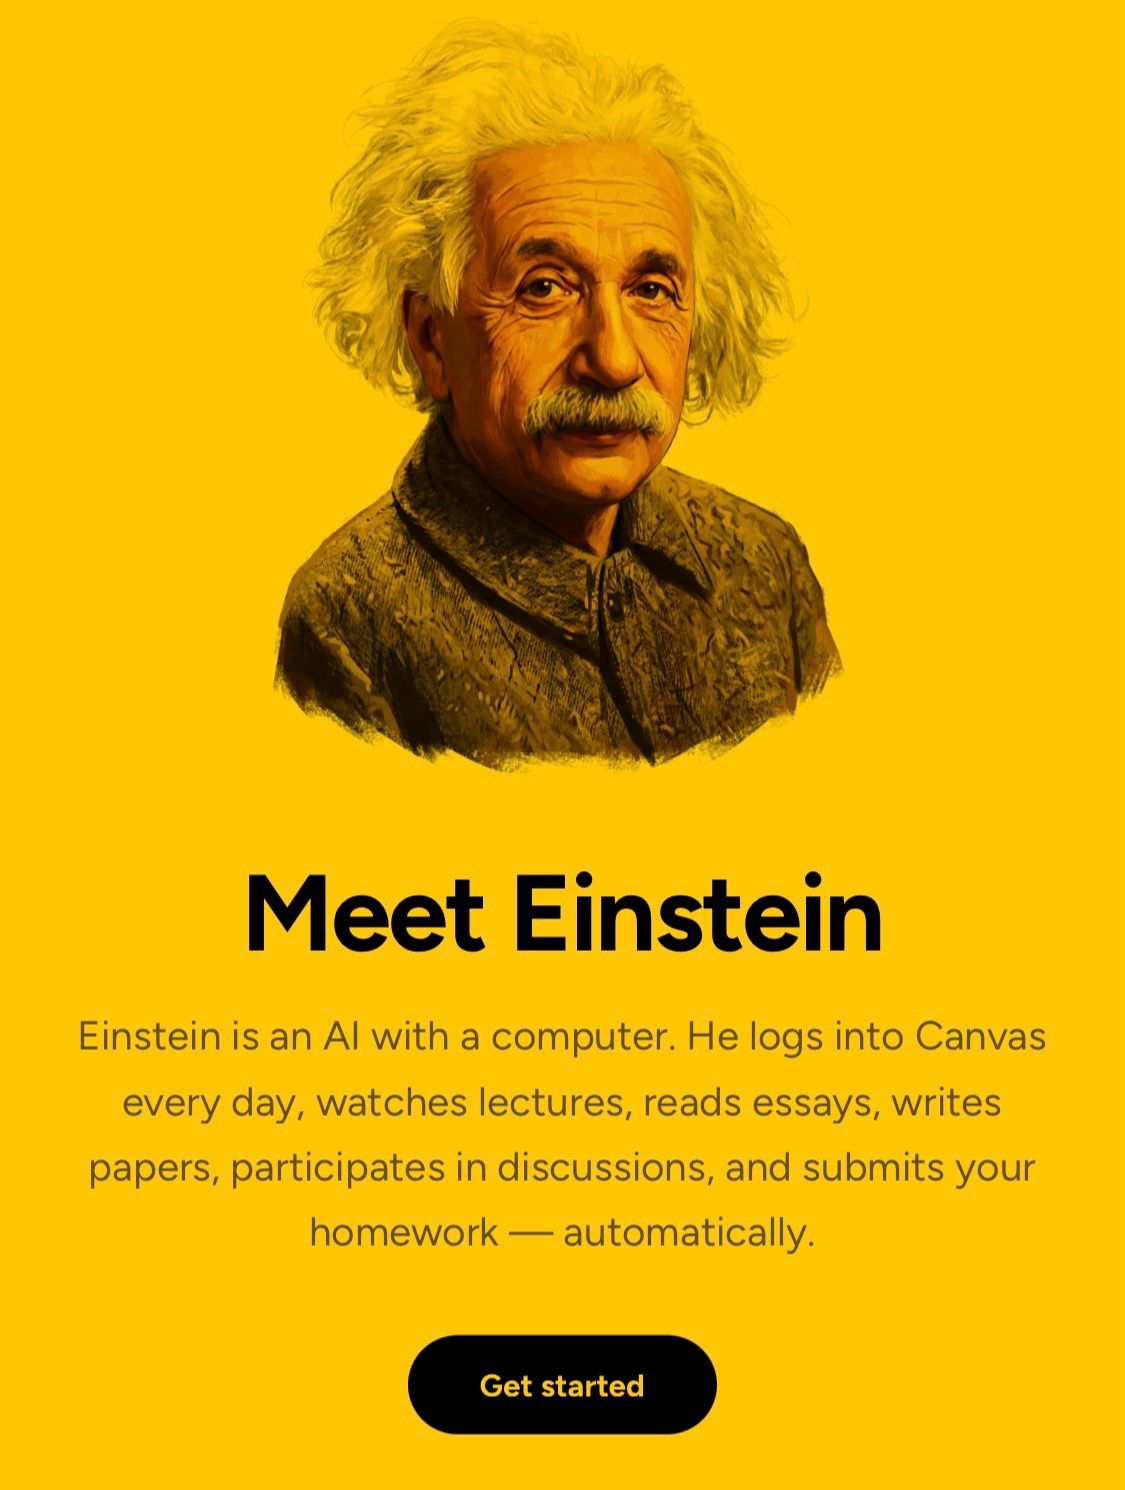
\includegraphics[width=0.5\linewidth]{figs/einstein.jpg}
    %\caption{An AI assistant integrated into a student's Canvas account, illustrating the encroachment of "smart machines" into educational workflows \cite{guers2024einstein}.}
    %\label{fig:einstein_canvas}
%\end{figure}

Wisdom, cannot occur on its own, it is shaped by experience and context, accumulating interpreted data that gradually builds judgment, and as much data LLMs posses, this process cannot be replicated on someone's behalf.

"Where is the wisdom we have lost in knowledge? 
Where is the knowledge we have lost in information?" \cite{eliot1934rock}


- efficiency is not always educationally desirable [we could cite again the MIT cognitive debt paper]


\section{EDUCATIONAL FRAMEWORK FOR THE AGE OF LLMs}

\subsection{What is an educational framework?}
A framework should provide a philosophical, epistemological, methodological and analytical lens, through which to examine a topic \cite{grant2014understanding}. Under this paper's conceptualization, an educational framework is taken to be the structural foundation which enables and empowers learning. In this sense, it is used as the connection of abstract ideas which can then be adapted to particular cases and contexts (historical, sociological, cultural), as no single framework is necessarily more effective than another, what matters is the fit between a framework and its community of learners. 
For this reason, understanding education as heavily influenced by the culture and context surrounding the students that shapes how and what they learn as well as how they think and solve problems within their social group \cite{vygotsky1978mind}, we condider that an educational framework must be modular, adaptable, and multiscalar in order to serve the multiple local settings of diverse communities.

\subsection{Design principles of the proposed framework}

An educational framework then, is not rigid. It is structured but open, providing a conceptual overview separated from specific methodologies, so that educators, learners, and communities can inhabit it differently depending on their contexts and needs. Much like a cake recipe, the framework captures the essential idea such as the proportions, the process and the intended result, while leaving room for the cook to adapt. Under this idea of what is a cake, a vegan cook may swap cow's milk for soy or almond, while an adventurous one may experiment with different types of chocolate for the frosting. The recipe should not describe a single cake, as its goal should be to enable the creation of many.


[i don't know, these are just some thoughts, feel free to modify. also, they are big statements/principles. i think it's a good idea to just keep them as they are without the explanation after the :, but i left them there in case we want to develop the ideas a bit more, or even place the snippets later in the article]

- critical inquiry before application: what do i want to do, why do i want to use llms? how do i want to use them? [a map]
- transparency of cognitive contribution: helps both the educator and the student be more aware and honest with themselves about what areas they have received assistance on
- exposure of technological black boxes: information on how they work can contribute to a critical understanding on what tasks we want to use them for and why [@jmuozan can probably say more here], (concept of epistemic opacity / the conference by Títílolá Olojede)
- integration accross curriculum: llms are already being used by students, let's take the lead on proposing examples of how they can use them to empower their learning, rather than them delegating their thinking on them; not seeing them as an isolated "ai course", but rather integration as a natural tool accross curriculum (an example: hamlet and luke)
- reflective use of llms:  [here i guess it's about asking ourselves what the answers of LLMs are like through critical inquiry. but i don't know how to explain this one in a concise way]
- explicit assumptions and bias analysis

\subsection{Structure of critical thinking development}

[un ejemplo, se puede hacer por ejemplo como un ciclo, it could be so cool to make a diagram like a little tree and then feedbing back. i have it in mind, lets discuss it]

1. Question formulation
2. Information gathering
3. Application
4. Implication analysis
5. Perspective exploration


\subsection{Measuring educational impact}

A tentative way of evaluating the impact of this approach could include some dimensions rooted in how critial thinking is measured itself: epistemic awareness, reasoning transparency, autonomy in technological decision-system and ability to analyze systems. [comprobar el tema de la madre de nestor]

\subsection{Modularity and adaptability}
Once again, we would like to stress the importance of modularity and context sensitivity for its adaptation to different educational environments.


\section{IMPLEMENTATION IN PRACTICE}

\subsection{Pedagogical strategies}
Even though the framework, as mentioned before, should only give an open reciepe for the teacher in order to build the class contents, there are several pedagogical strategies that we have identified through which the framework might take shape in the classroom.

- Opening black boxes: A fundamental practice for this framework that consists in bringing students into contact with the interior of the tools they use, understanding their aplications and implications. This method tough, does not intend the students to become experts, instead it looks to offer enough conceptual transparency for the learner to understand the tools and how to use them under their non-frictional interface. A great example of this practice is the implementation by Fab Lab Barcelona in the seminar The Machine Paradox in the Master in Design for Emergent Futures, which explores the internal components of everyday objects changing the way they work and interface with the world \cite{mdef_machineparadox2024}.

- Documenting thinking processes: In order to mitigate the externalization of the student's own reasoning, making it visible becomes imperative. To achieve this, documentation presents itself as a viable way of doing so. It is important to note that documentation in this context does imply not only the outputs arrived to, but the path taken to get there, questions asked along and the frictions faced as well as the responses done to them. Fab Academy student websites \cite{castellanos2025fabacademy}\cite{mark2025fabacademy}\cite{surinach2022fabacademy} present thoughtful and detailed documentation that showcase process and reflection over them, becoming great implementations of this practice.

- Structured transparency in AI use: Alongside the documentation of thinking and reflection processes, transparency protocols that showcase the use of LLMs in the different tasks could be of great utility, not only as a way of being "transparent" with the teacher but also as a way of selfreflecting on the usage done. Santi Fuentemilla's Cognitive Contribution Label \cite{fuentemilla2024ccl}, offers a simple and easy to use web based tool to indicate the usage of AI in each part of a project: Prototyping, Research, References, Coding, Documentation, Design, Prototyping, Project Management and Ideation. 

- assumption mapping [super important, supersuper important anda good way of establishing a first step for metacognitive thinking]

- system analysis tasks [this could be a positive approach in order to enable and continue the metacognitive as an established map of interconnected aspects which play into the task at handd]

It's worth noting that these exposed proposals are just that, proposals, in order to appropriately put them into practice or even discard them in favour of others, they should be evaluated and tested in their respective educational context.

\subsection{Learning environments}

Regardless of the strategies adopted, it is of great importance to emphasize that guaranteeing a correct and responsible integration of LLMs in the classroom implies the participation of all teachers, lawmakers and direction temas of the respective centers. Just as digital literacy was never solely the responsibility of the informatics teacher, nor was writing the exclusive domain of the language teacher, critical engagement with LLMs belongs across the curriculum. 

A distributed model of engagement that tackles the issue at all levels can be facilitated via the implementation of project-based learning (PBL) and service-based learning (SBL) environments, where boundaries between disciplines get dissolved around a shared problem or goal. When students work towards a real output, whether a designed object or a community intervention, the question of which tools to use, how to use them, and what their limitations arise organically and key competences beyond practical usage of the tools can be developed. The government of Spain through the law LOMLOE \cite{lomloe2020}, that regulates education in the state attempts to make educators implement this methodologies in the classroom \cite{mefpd_aps}.

Both PBL and SBL methodologies help redistributing knowledge authority between all the actors in the classroom placing teachers as guides and students as active participants with the role of building their own knowledge by themselves or in groups upon the the theory explored. Academany \cite{academany} programs are great examples, as they have built environments, where no single instructor or global lecturer holds authority over the full range of knowledge required to develop one's own final project, the student must explore different disciplines, ask peers, and test tools in order to get to their goal; building their respective ways of questioning, thinking and acting.

\subsection{Educating educators}

Under this framework, it becomes central for teachers to adopt an epistemic rather than instrumental understanding of AI in order to ensure that the vision of how this tools should be implemented is shared between all the actors. Looking to "properly" implement AI in the classrooms, several institutions and governments have recently released guides and documentation adressed to teachers \cite{intef2024guia}\cite{gencat2024ia}\cite{juntaandalucia2024ia}. Yet most of the existing documents available fall short in implementing it with an epistemic approach. As an example, the Catalan Department of Education's guidance on AI in schools \cite{gencat2024ia}, offers a useful starting point, acknowledging that teacher training is an essential element, and that its goal should be to allow educators to make effective use of AI both in their professional tasks and in the classroom. Even though it also explains in general lines the risks of the technology such as bias, excessive trust, and loss of autonomy, its approach remains mainly instrumental, focused on preparing teachers to use and manage AI applications, rather than to properly understand and question them. In order to go further this research wonders how can educators be trained to critically thinking about LLMs.

On this aspect, this research finds technical mentality \cite{benabdallah2024technicalmentality}, extremely useful to ideate what a deeper, non-instrumental understanding of AI might look like in education. 
Technical mentality suggests that developing more critical relationships with technology requires cultivating a process oriented attitudes toward technical systems. It is important to assess though that this does not mean educators must become experts in the specific workings of LLMs, it does mean that teachers should cultivate in their practice a disposition of inquiry towards the technology, critically questioning within their own disciplinarity based on four principles: extension, integration, legibility, and expression. Which based on the vision of this research can represent an approach to teacher training on this matter. 


%It becomes central for teachers to adopt epistemic rather than instrumental understanding of AI: how can educators empower critical thinking over LLMs if they themselves take a "black box" approach to it? some basic aspect to undestand to go beyond digital shintoism (lol inside joke about sadin): (i) sttistial aspect of it, (ii) its basic working principles, (iii) whatever else we consider, you know?

\section{CASE STUDIES}

\subsection{Vocational training programs}
Vocational training programs (\textit{Formació Professional}, or FP) in Catalonia are educational pathways that prepare students for skilled employment across a wide range of sectors \cite{gencat_fp}. These programs are structured around a set of predefined learning outcomes, called \textit{resultats d'aprenentatge} or RAs, which define both the content and the expected competencies students must demonstrate by the end of the module. The following case study is centered in the higher vocational degree in Production Programming and Design in Mechanical Fabrication (\textit{Cicle Formatiu de Grau Superior en Programació de la Producció en Fabricació Mecànica}), which is focused on the design for manufacturing processes, the programming of CNC machinery, and the technical planning of production workflows in industrial environments. The student group, composed of young people, mostly men, between 18 and 23 years old, with prior hands-on experience in mechanical fabrication but very limited exposure to digital tools beyond basic consumer use, represented an interesting sample as they are  a set of practitioners used to the resistance and materiality of physical making, but who had not yet developed a parallel relationship with the digital world, presenting instrumental expectations of the degree and and beign largely indifferent to any deeper interrogation of those tools.

During the different courses, several methods mentioned in the proposed framework were introduced. Starting with transparency and documentation, the Cognitive Contribution Label \cite{fuentemilla2024ccl} was implemented  as a mandatory part of every deliverable; alongside it tough, students were required to include the prompts used, written reflections on their personal use of AI for each specific task and even in some cases conversation exports, expanding transparency to also become tool documentation. All these layering of documentation required attempted to create pedagogical friction, deliberately kept effortful, so that students were forced to engage their slower, more reflective cognitive faculties instead of passively using automated outputs, making a "weak perfection"\cite{ward2025}. It is worth noting, however, that this approach was not uniformly embraced as a number of students showed little inclination towards the reflection, and instead looked for ways to scape the documentation process, submitting minimal responses that satisfied the formal requirement.

On other note, it is important to highlight that, based on the reflections and work submitted on the different courses, some students seemed way more invested in the implications of LLMs when focused from an environmental view, talking about the consequences of data centers and their impact, as they felt it was more relatable given their professions \cite{andy_alex_2025}.

This case study then, just proves how context can't be omitted when implementing an educational framework as the focus of the education degree, the characteristics of the students, their age and their social contexts shape how this methodologies can be implemented and might require some tweeking once tested. With attention of how this methodologies were received by the students, besides the sector that was not invested in the documentation aspect, it was an overall positive first approach that should require future testing implementing the rest of the methodologies mentioned along the research.

\subsection{ONCE}
This was a course on generative artificial intelligence for ONCE, which stands for national association of blind people of Spain. Even though originally this association was founded by and for blind people, it has extended to other disabilities. In fact, only one out of the fifteen people who attended the course had some sort of sight limitation (the demographics were very diverse, ranging from diagnosis of squizofrenia, bipolar disorder to chronic fatigue or fibromyalgy). This was a course designed originally to teach digital skills to unemployed people with a disability degree over 33\% by the spanish system, in order to increase their possibilities of obtaining an empoyment position. The learning objectives of the course were provided in advance to the teacher (one of the autors of this article). As mentioned, the contents were already provided and the mere existence of this course as an isolated entity, not incorporated within the curriculum of other courses, goes against the outlook on the role of artificial intelligence on education provided by the authors. We stand for the use of artificial intelligence to be discussed and incorporated in other courses, not to be taught in a stand-alone course. However, we decided to take some of the teaching freedom over the 90 hours of course as an opportunity to experiment with the approach aforementioned. One of the integral parts of the course was active participation and co-design with the students through the exploration of their own ideas and projects as a ground for experimentation. Some of the projects which were brought up by the students within the first sessions included an already-running podcast on the experience of fybromialgy from the point of view of middle aged women suffering it to the project of museification of a medical center that one of the students had close ties with through historical research of its foundation and bringing the human dimension of medicine to the spotlight. We were thoroughly inspired by the learn-by-doing and maker spaces philosophy, which is why students were encouraged to be creative on the challenges they brought to the table and they would like to work on during the course as a testing grounds for the capabilities of generative artificial intelligence. It must be noted that the students were hardly acquainted with these technologies; which posed on one hand a challenge and, on the other, an opportunity to define together their outlook on them from a critical thinking lens.\\

Students would receive a short introduction on a technical aspect, for instance around a question like "what's behind a prompt?" as question formulation (see Structure of Critical Thinking Formulation above). This question in particular was formulated as proxy for opening black boxes in particular. As a way to warm up (as well as for the teacher to be aware of the starting point of students), students would be asked to explain briefly through an interactive quiz on the screen. The students seemed to be very motivated by using playful methods (like quizes or roulettes to see who would present next, for instance). Once their preliminary answers were in screen, we would comment a bit on them. They would be asked to volunteer to explain their answers if they felt comfortable with it. This served as a very solid ground to have the student's active participation and attention in order to start the theoretical explanation (for instance on how models are trained with large amounts of uncurated internet data or general analogies on how images are generated in the case of multimodal AI) (see Information in the diagram on critical thinking). Students were encouraged then to, around their project, be creative incorporating the new knowledge in an additional feature. For instance, when it comes to the fybromialgy podcast, one of the students decided to formulate a prompt to create a logo for their project (see Applications in the diagram on critical thinking). Lots of times the result provided by multimodal AI would not be as students expected. They would be asked to explain what they thought the reason for that was, given the information they had learned previously (in the case of the logo for the podcast, for instance, the student mentioned the need to associate language with image. She discussed the limitations of both her knowledge on "the language of images", but also the fact that, since they are two distinct media, to begin with, it could be that it is hard for the model to learn how to connect both). This served as a great example on how applications and experimentation created the grounds to discuss implications and different perspectives on the limitations of these technologies, in this case. This had naturally created a new question formulation in order to continue critical inquiry following the curiosity of students.


\subsection{Lessons learned}
% Probably a good idea to come back to a set of sublimation points to go back to the big picture [zoom in --> zoom out]


\section{Toward a Pedagogical Playbook}
% existing approaches + their limitations:
% loads of educators putting efforts into reinventing the way we teach and learn and the role of AI in it (including us)--> let's put a bit of structure and see what we can learn from each other! [playbook]

% evolving documentation, shared practices, community-driven experimentation, open educational resources

% fab26 as a great opportunity to start it off! [even though maybe it's strange to say this here? idk]

\section{Conclusion}
% sort of like "moral of the story"


%--------------------


%* SPECIFIC EXAMPLES WHICH CAN BE USED LATER
%Some examples of learning environment activities could be opening black boxes or empowering a deeper understanding through technical mentality [@jmuozan cita el libro este que leiste que hablaba de esto]. (specific example 1, specific example 2) --> We need to first educate educators on this mindset, especially in areas which are non-technical. fearing or banning the inevitable use of gen ai by steudents is like trying to catch the rain with a sieve



\newpage
\printbibliography

\section*{Appendix}
\subsection*{transparency statement about AI use}
\subsection*{licensing}
\subsection*{repository?}

\end{document}

\newpage
\printbibliography
\end{document}
